\documentclass{article}
\usepackage[T1]{fontenc}
\usepackage{lmodern} %sets the font
\usepackage{amsmath}
\usepackage{graphicx} % Required for inserting images
\usepackage{xcolor}
\pagecolor[rgb]{0,0,0} %black
\color[rgb]{0.9,0.9,0.9} %grey
\usepackage{hyperref}
\hypersetup{
    colorlinks=true,
    linkcolor=blue,
    filecolor=magenta,      
    urlcolor=cyan,
    pdftitle={Overleaf Example},
    pdfpagemode=FullScreen,
    }
\urlstyle{same}
\title{Network Science Notes}
\author{Ben Hizak}
\date{January 2025}
\setlength{\parindent}{0pt}
\begin{document}

\maketitle 


\begin{table}
    \centering
    \begin{tabular}{l}
        I am looking for help maintaining this notebook. If you are interested please contact benhizak@gatech.edu\\
    \end{tabular}
    \caption{Caption}
    \label{tab:my_label}
\end{table}
\section{Terms}

\subsection{Graph Elements / Notation}

\begin{table}
\centering

\begin{tabular}{|l|l|l|l|}
\hline
\multicolumn{2}{|c|}{\textbf{Network Science}}& \multicolumn{2}{|c|}{\textbf{Graph Theory}}\\
\hline

\hline
Network  && Graph $G = (V, E)$ &\\
\hline
Node $N$ &$n$ Nodes& Vertex $u \in V$ &$n$ Vertices\\
\hline
Link $L$ &$m$ Links& Edge $(u, v) \in E$  &$m$ Edges\\
\hline

\end{tabular}

\end{table}

Terms Network Science vs. Graph Theory

\subsection{Graph Attributes (Parameters, Properties)}
\begin{description}
    \item [Neutral Networks] networks in which there is no correlation between degrees of any two nodes $u$ and $v$
    \item[$k_i$ Degree] The number of nodes to which a given node is connected. The sum of degrees is $sum(degrees)=2*|E|=2m$.
    \item[$\overline{k} $ or $\langle k\rangle$ Average Degree]  $\overline{k}= \frac{1}{n}\sum\limits_{i = 1}^N {k_i } =\frac{2|E|}{n}=\frac{2m}{n}$
    \item[$p_k$ Degree Distribution] shorthand for $Probability (deg(v) = k)$ or $P(k)$ the probability that a randomly chosen node will have degree $k$ \\
    Undirected:             $L = \frac{1}{2}\sum\limits_{i = 1}^N {k_i }$ \\
    Directed: $L = \sum\limits_{i = 1}^N {k_i^{in} }  = \sum\limits_{i = 1}^N {k_i^{out} }$
    \item [Edges (E)]the count of edges is denoted by m
    \item[Maximum Edges]  $L_{max}={\binom{n}{2}}=\frac{n(n-1)}{2}$
    \item [Density] the number of edges relative to the $L_{max}$ the maximum possible of edges. Expressed $\frac{|E|}{L_{max}} =  \frac{|E|}{\binom{n}{2}}$

m = $p\cdot\frac{n(n-1)}{2}$
\end{description}
\paragraph{Average nearest neighbor degree }
To calculate $k_{nn}(k)$ we calculate the average value of $k_{nn}(k)$ for all nodes v with $k(v)=x$

\begin{figure}
    \centering
    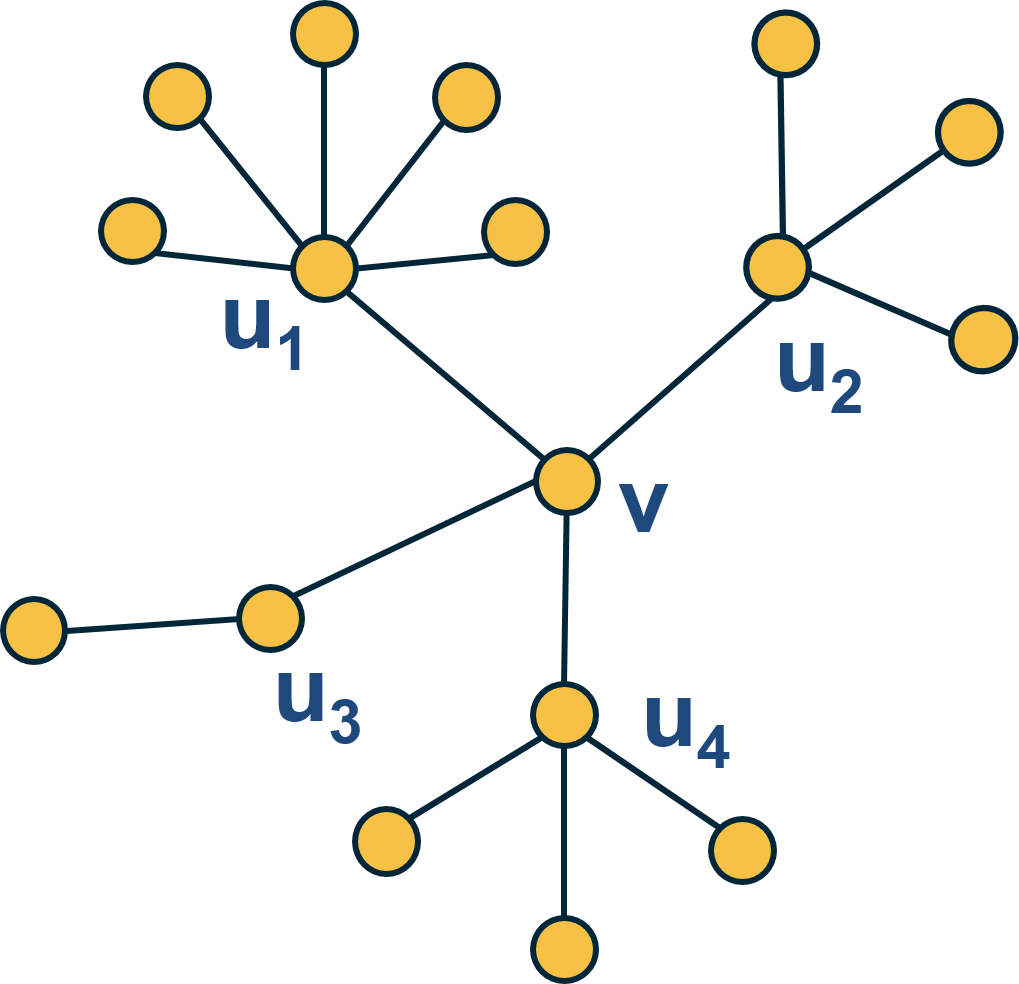
\includegraphics[width=0.5\linewidth]{k-neighbor-example.png}
    \caption{formula: $\overline{k_{nn}}(v)\:=\frac{\:1}{k(v)}\sum\limits_{i=1}^{k(v)}k(u_i)=\frac{6+4+2+4}{4}\:=\:4$}
\end{figure}

\subsection{Adjacency Matrix and List}
The adjacency list representation requires n+2*m space because every edge is included twice. 
\textbf{TODO adjacency matrix}
\newpage
\section{Neutral Network}
Definition: the Degree of any two notes is not correlated.
\textbf{Most networks are not Neutral}
$k_{nn}(k)\:=\:\overline{k}+\frac{\sigma_k^2}{\overline{k}}=\bar{k}_{nn}$
\newpage
\section{The \textit{G(n,p)} model (ER Graphs) Erdős–Rényi}
This is the simplest random graph. It is not the same as the $G(N,L)$ graph, which has a fixed number of random links.
\subsection{Construction}
\begin{description}
    \item [n] Nodes
    \item [p] the probability any two nodes are connected 
\end{description}

\subsection{Properties}
Note how the LCC suddenly 'explodes' when the average node degree is greater than 1. This is called a phase transition. 
\begin{figure}
    \centering
    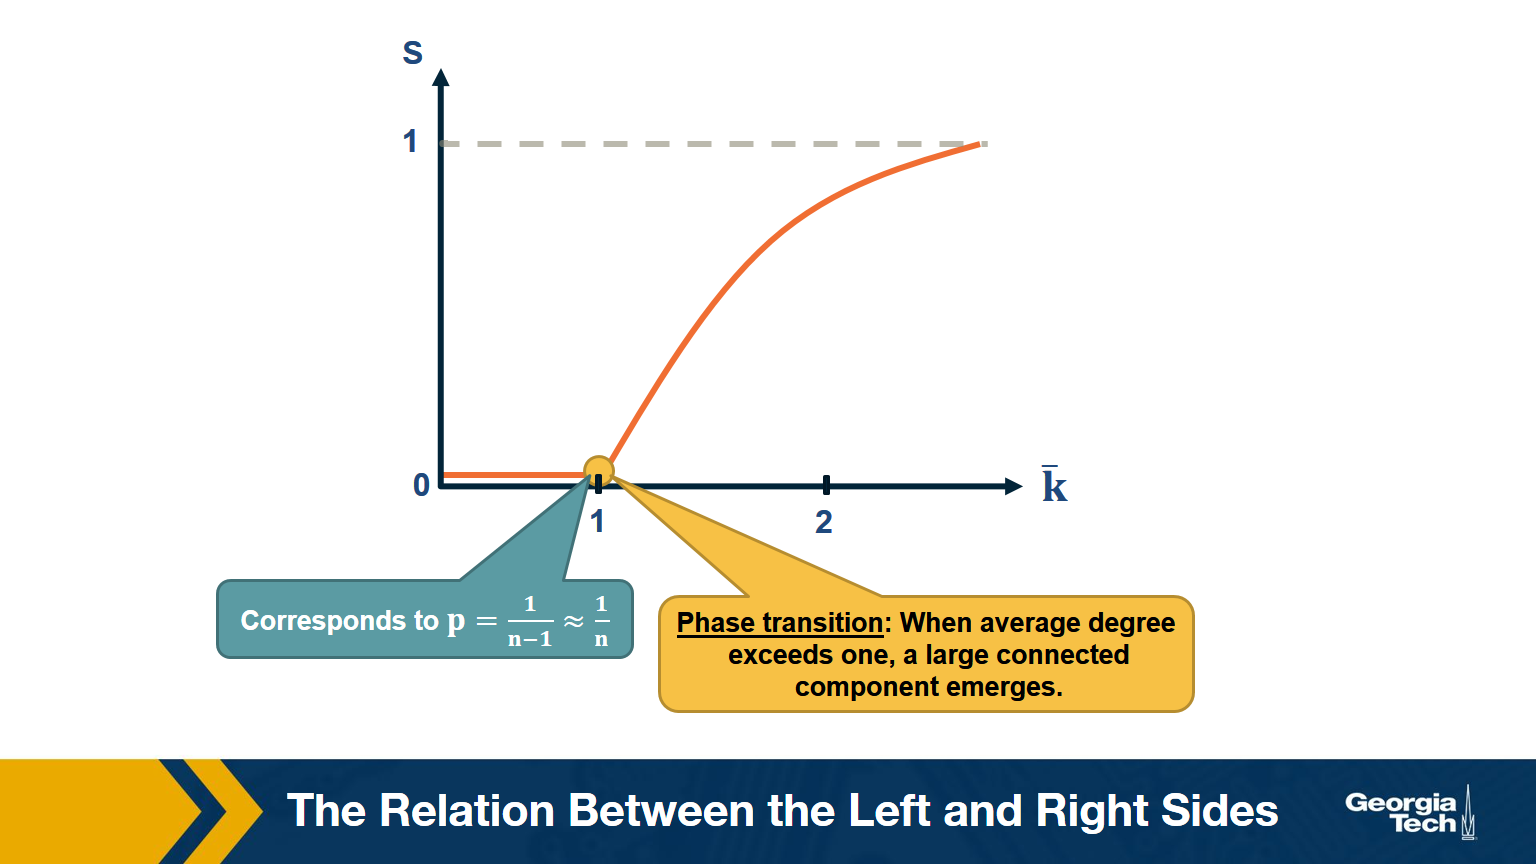
\includegraphics[width=1\linewidth]{lcc-explosion.png}
\end{figure}
\begin{description}
    \item [Degree Distribution]  $p_k\:=\:e^{-\overline{k}}\cdot{\frac{\overline{k}^{k}}{k!}},\:k=0,1,2,\dots$
    \item [average edges] $p\cdot{\binom{n}{2}}$
    \item [edges] expected number of edges is  $|E|=p\cdot\frac{n(n-1)}{2}$
    \item[LCC] Largest Connected Component
    \item[Degree = Link Count $P_L$] = \\$ P(Link Count = L) =( {\begin{array}{*{20}c} {\frac{{N(N - 1)}}{2}}  \\ L  \\ \end{array}} )p^L (1 - p)^{\frac{{N(N - 1)}}{2} - L}$
    \item [S] the probability that a node belongs to LCC\\
    $\overline{S} = S-1$ represents the probability that a node is \textbf{not} connected to a LCC
    $\overline{S}\:=\:((1-p)\:+\:p\cdot\overline{S})^{n-1}$\\
    $1-p$   Probability that a node is not connected to a randomly chosen other node.\\
    $p\cdot\overline{S}$ Probability that the node connects to a node \textbf{not in} the giant component.
    \item [average node degree] $p \cdot (n-1) $
    \item [average neighbor degree] at a $G(n,p)$ network is\\
    $\overline{k_{nn}}=\overline{k}\:+\:(1-p)$ using the Binomial distribution) or\\
    $\overline{k_{nn}}=\overline{k}\:+\:(1-p)$ using the Poisson approximation when $p\ll1$
\end{description}
\textbf{Question: how large should $p$ (or $k$) be so that the LCC covers all network nodes?}

Answer: The probability that a node does \textbf{not} connect to any node in the LCC $(1-p)^{S \, n}\approx(1-p)^n\:$if$\:S\approx1$

The expected number of nodes not connecting to LCC:
$\:n\cdot(1-p)^n\:=\:n(1-\frac{np}{n})^n\approx n\cdot e^{-n\cdotp}$

\subsection{classification of Networks}
\begin{description}
    \item[Scale Free] (TBC)
    \item[Neutra] (TBC)
\end{description}
$P_{edge}(k)= $Probability(given edge has degree k)$=\frac{kP(k)}{\overline{k}}$
Limit Definition of Exponential Function $(1-\frac{x}{n})^n\approx e^{-x}$
\subsection{links}
\href{https://en.wikipedia.org/wiki/Erd%C5%91s%E2%80%93R%C3%A9nyi_model}{wikipedia}\\
\href{https://en.wikipedia.org/wiki/Binomial_distribution}{Binomial distribution}\\
The Puissant distribution is a good approximation when $n>1,000$

\section{Calculating Random Walks}

\subsubsection{\textbf{Key Definitions}:}

\begin{enumerate}
    \item \textbf{Graph Representation}:
    \begin{itemize}
        \item Let the graph have $n$ nodes, and the weight of the edge between nodes $i$ and $j$ is $w_{ij}$ 
        \item The graph is undirected, so $w_{ij}$ = $w_{ji}$ 
    \end{itemize}
    \item \textbf{Weight Matrix ($W$)}:
$W$ is an $n\times n$  matrix where$ W[i,j]=w_{ij}$, the weight of the edge between $i$ and $j$. If there is no edge, $W[i,j]=0$.
    \item \textbf{Degree Matrix ($D$)}:
$D$ is a diagonal matrix where $D[i, i]$$ = \sum\limits_{j} W[i, j]$ is the total weight of the edges connected to node $i$.
    \item \textbf{Transition Matrix ($P$)}:   $P=D^{-1}W$ where $P[i,j]$ is the probability of transitioning from node $i$ to node $j$ in one step.
    \item \textbf{Initial State ($\pi_0$)}:
For a uniform starting distribution, $\pi_0=\frac{1}{n}\textbf{1}$ where $\textbf{1}$ is an $n$-dimensional vector of all 1s.
\subsection{Steps to Compute the Random Walk:}
\paragraph{1. \textbf{Construct the Transition Matrix ($P$)}:}
Compute $P=D^{-1}W$ . This normalizes the rows of $W$ so that the sum of probabilities in each row is 1.
\paragraph{2. \textbf{Perform the Random Walk}:}
\begin{itemize}
    \item At each time step $t$, the state distribution $\pi_t$ is updated as: $\pi_t=\pi_{t-1}P$ 
    \item For $t=1,2,3,…$ repeat the matrix multiplication to compute the distribution of the random walk over time.
\end{itemize}
\paragraph{3. \textbf{Stationary Distribution (Long-Term Behavior)}:}
\begin{itemize}
    \item For large $t$, the random walk converges to a \textbf{stationary distribution} $\pi_\infty$, satisfying: $\pi_\infty P=\pi_\infty$
    \item Solve for  $\pi_{\infty}P=\pi_{\infty}$ as the dominant eigenvector of $P$ corresponding to eigenvalue $1$, normalized so that $\sum\limits_i^{}\pi_{\infty}[i] = 1$.
\end{itemize}
 
\end{enumerate}

\section{Power Law Networks}
This means that the \textbf{maximum degree in a power-law network increases as a power-law of the network size n. If $\alpha=3$ the maximum degree increases with the square-root of n.} 
$k_{max} = k_{min} \, n^{1/(\alpha-1)}$
\section{Resources}
\href{https://gatech.instructure.com/courses/433540/modules}{Course Modules}
\href{https://cazabetremy.fr/Teaching/CN2021/CheatSheet/CN_CS_introduction.pdf}{Cheatsheet}
\href{https://www.albany.edu/~ravi/pdfs/sol_hw2.pdf}{CSI 445/660 – Network Science – Fall 2015}

\end{document}
